\chapter{Architectural design} \label{chap:architectural}


\section{Overview}
This chapter, arguably the longest of this document, analyses different aspects of the architecture of myTaxiService system. In \cref{sec:highlevel} we give a high level description of the structure of the system; inevitably this section will be pretty theoretical.

Then in \cref{sec:componentView} we focus on the components of the system. With the word \emph{component} we refer to a software package, a web service, a web resource, or a module that encapsulates a set of related functions. The interfaces between the components are fully analysed in \cref{sec:componentInterfaces}. The deployment view in \cref{sec:deployment} provides further details on the structure of the various parts of the system, in opposition to the focus on the communications between them . 

In the runtime view (\cref{sec:runtime}) we show the behaviour of the system in case of a request and a reservation. 

Finally, \cref{sec:styles} and \cref{sec:decisions} are meant to give further details and explanations about our design and architectural choices.

In the whole chapter, we will make extensive use of UML diagrams, UML being an agreed and relatively easy to understand language.


\section{High level components and their interaction}\label{sec:highlevel}

%[JavaEE architecture > see Quinton]

%[here you can introduce the high level components of your architecture (in our basic example in the slides about design you find these in slide 7) and describe the main interaction between them (no details here. You can say why some components talk to each other, why, if the communication is synchronous or asynchronous, any other info you think is useful at this point).]

For our myTaxiService ecosystem, we will adopt the Java Enterprise Edition (Java EE) application model for enterprise applications. This will allow the design, building and production of a solid, fast and reliable system, with a special focus on money and resources. 

\begin{figure}
	\centering
	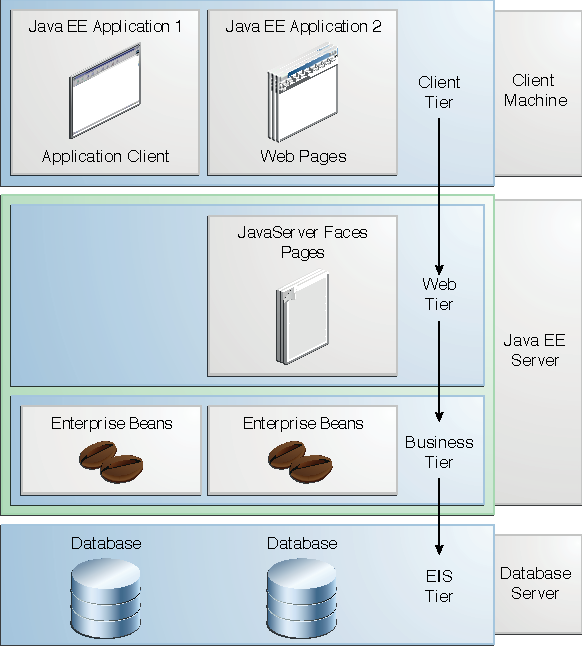
\includegraphics[width=0.85\textwidth]{img/JEETT}
	\caption{High level architecture.}
	\label{fig:jeett}
	%TODO Source!
\end{figure}

The Java EE platform uses a distributed multitiered application model, shown in \cref{fig:jeett}. Application logic is divided into components according to function (these will be detailed further in the chapter), and the application components that make up a Java EE application are installed on various machines depending on the tier to which the application component belongs. \Cref{fig:jeett} shows the model we will adopt, which consists of four tiers:

\begin{description}
	\item [Client tier] it contains all the components which run on the client machine (applications, web pages); in our case myTaxiWeb web pages, and myTaxiApp, myTaxiAssist mobile applications are the clients. These are all \emph{thin clients}, which means that they do not directly query the database, nor execute complex operations. 
	
	\item [Web tier] the components of this tier run on the Java EE server; this tier is intended to mange the data flow between clients and Java EE server and between server components and the database.

	\item [Business tier] this tier, which runs on the Java EE server as well, contains the so called \emph{enterprise beans}. Enterprise beans handle business code, which is logic that govern myTaxiService system; to do so, they also retrieve data from storage, processes it (if necessary), and sends it back to the client program.

	\item [EIS tier] this tier, typically, handles EIS\footnote{EIS stands for Enterprise information system.} software and includes enterprise infrastructure systems, such as enterprise resource planning (ERP), mainframe transaction processing, database systems, and other legacy information systems. In our specific case, Java EE application components might need access to enterprise information systems for database connectivity.
	
\end{description}













\clearpage%TODO Remove.
\section{Component view}\label{sec:componentView}
[BCE diagram? controllers as components?]

[here you have a refinement of what you have in Section 4.B and identify sub-components. For instance, the diagram in slide 6 could be a diagram showing a  component view]

Diagramma che presenta i vari component di cui sarà costituito il sistema, per comodità sono suddivisi nelle varie applicazioni che andranno a costituire lo stesso e in subsystem.
Vengono inoltre presentate le interfacce “provides” and “requires” che ogni component mette a disposizione (o richiede) per poter comunicare con gli altri component.
È indicata la modalità di comunicazione tra le varie applicazioni, mentre sono escluse, per maggiore chiarezza, tutte le connessioni di utilizzo tra le interfacce esterne ai subsystem.
Un component che con un’interfaccia di tipo “provides” offre un modo di interagire con lo stesso, mentre con l’interfaccia “requires” evidenza la necessità di interagire con un altro component. Maggiori dettagli sulle interfacce saranno forniti nella sezione 4.F (mi pare).
Particolare nota al subsystem EJB Container, che contiene quei JavaBeans ritenuti indispensabili per il corretto funzionamento del sistema, tra i quali Java Server Faces, lato server del web client, e tutte le funzionalità offerte da Java Persistence API (nel diagramma è indicato come JDBC, provvederò a correggere, ricordamelo!), per l’utilizzo del DB MySQL.

\begin{figure*}
	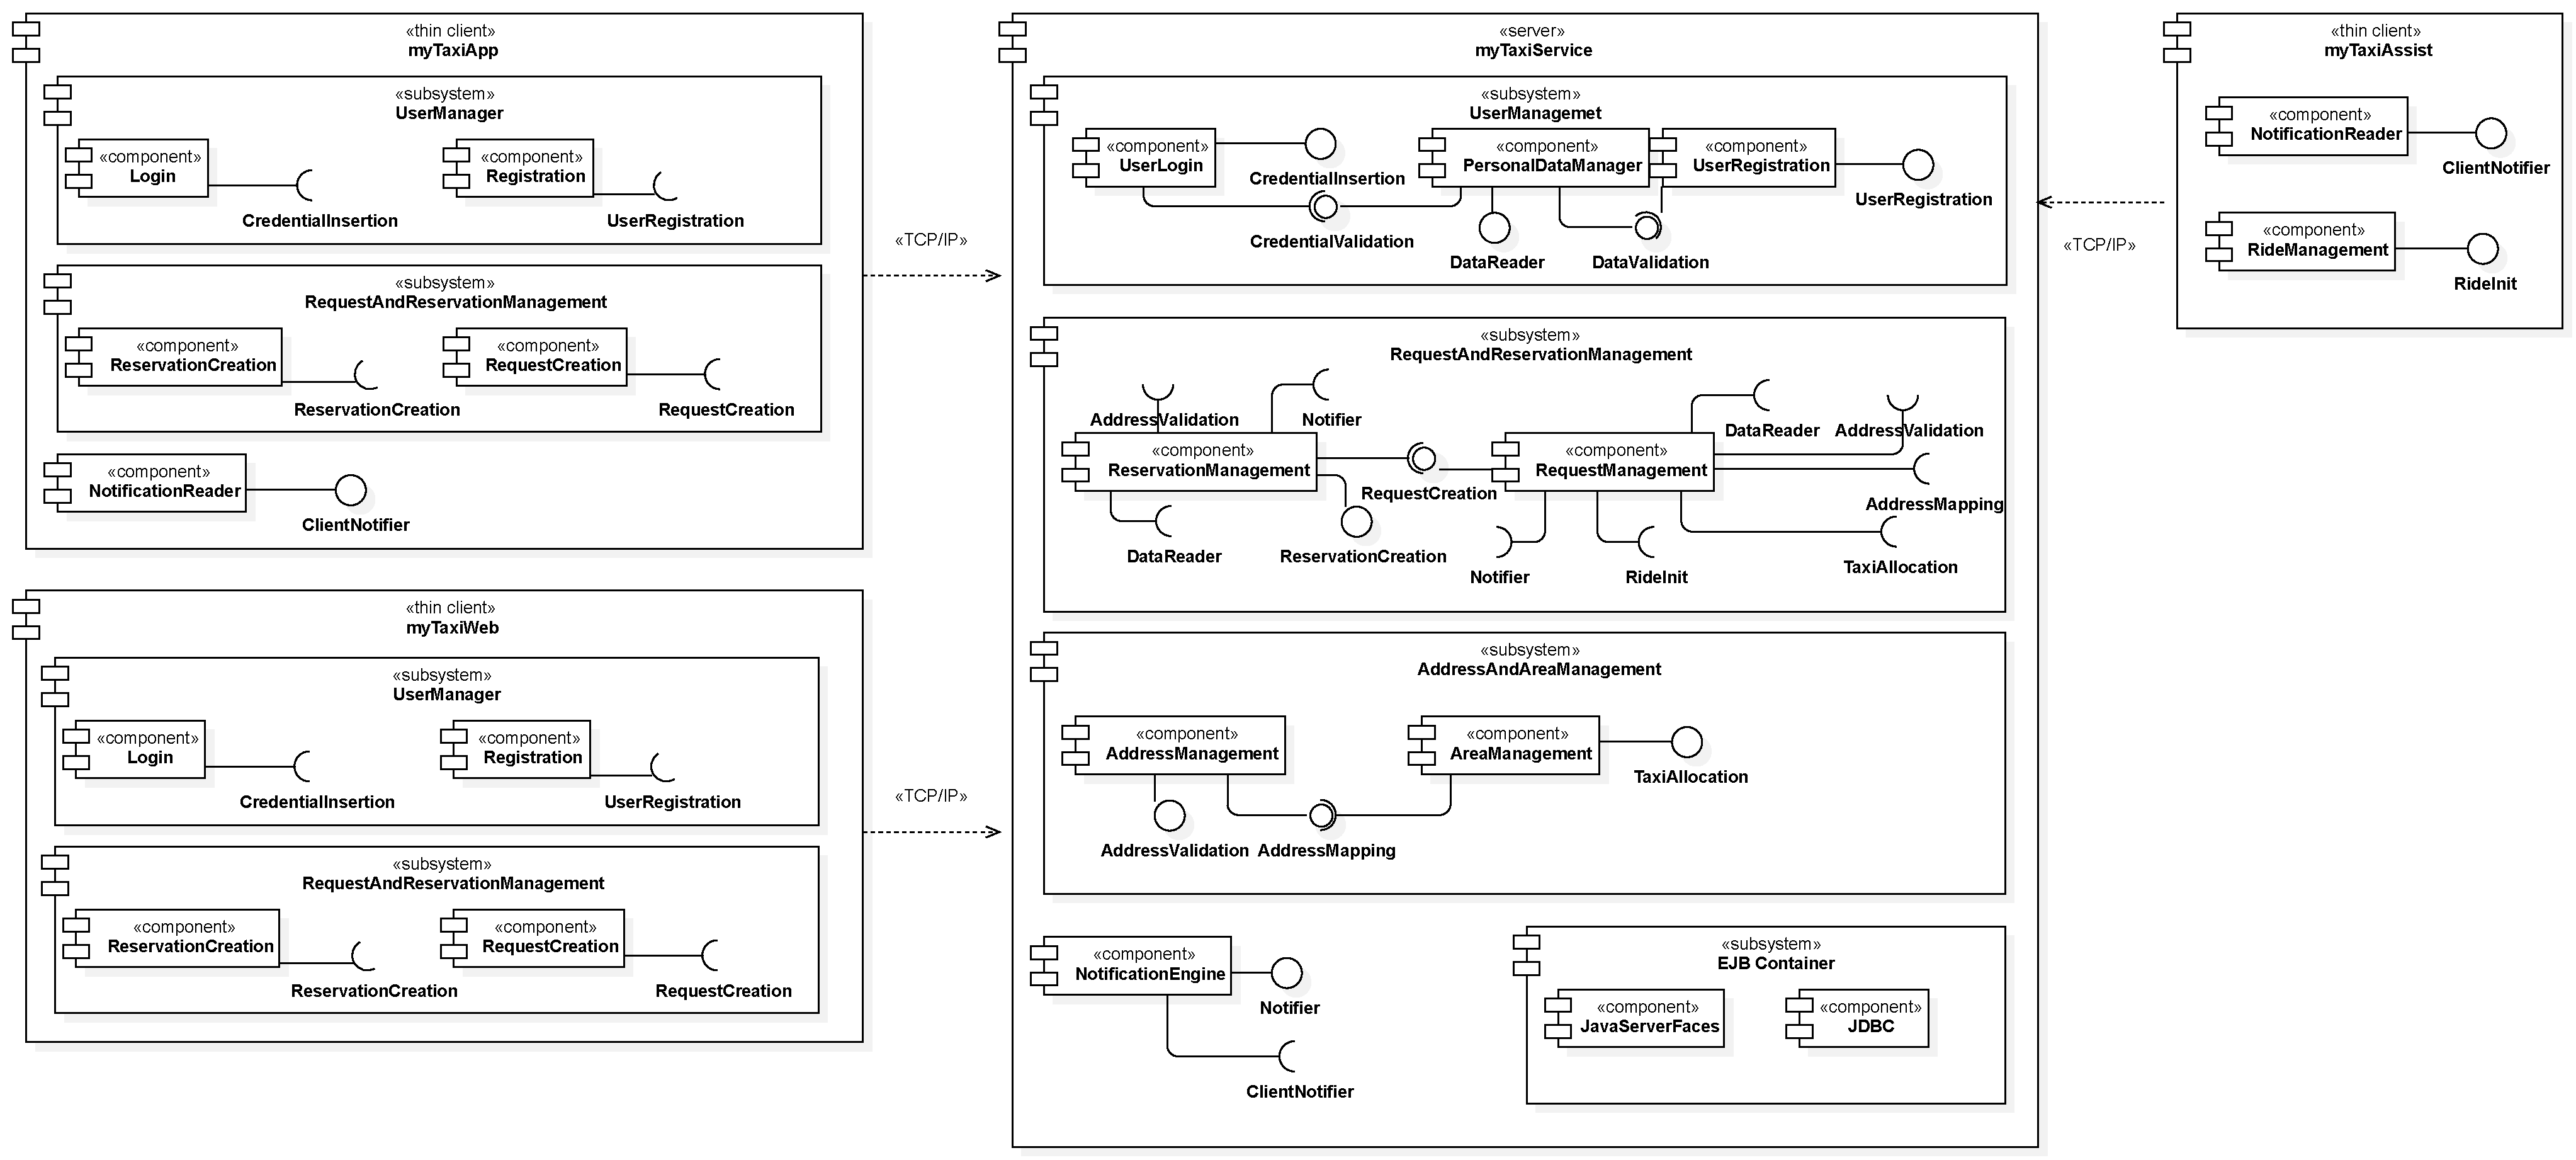
\includegraphics[width=\textwidth]{img/ComponentView__ComponentDiagram_1}
	\caption{Component diagram.}
	\label{img:component}
\end{figure*}















\clearpage%TODO Remove.
\section{Deployment view}\label{sec:deployment}
[this is what you have in slide 8, that is, the identification of the artifact that need to be deployed to have the system working]

Ogni nodo del DD indica un sistema hardware separato. Oltre ai Client, di diversi tipi, è prevista una macchina server che offra le funzionalità del sistema, mentre una seconda macchina server che funzioni solo da Persistance Server.
Sono inoltre indicati i subsystem che andranno ad essere deployati sulle varie macchine e l’interazione tra essi. Si è voluto specificare di alcuni la loro particolare funzione (non mi piace il termine), evidenziato il fatto che si tratti di eseguibili o di servizi.


\begin{figure*}
	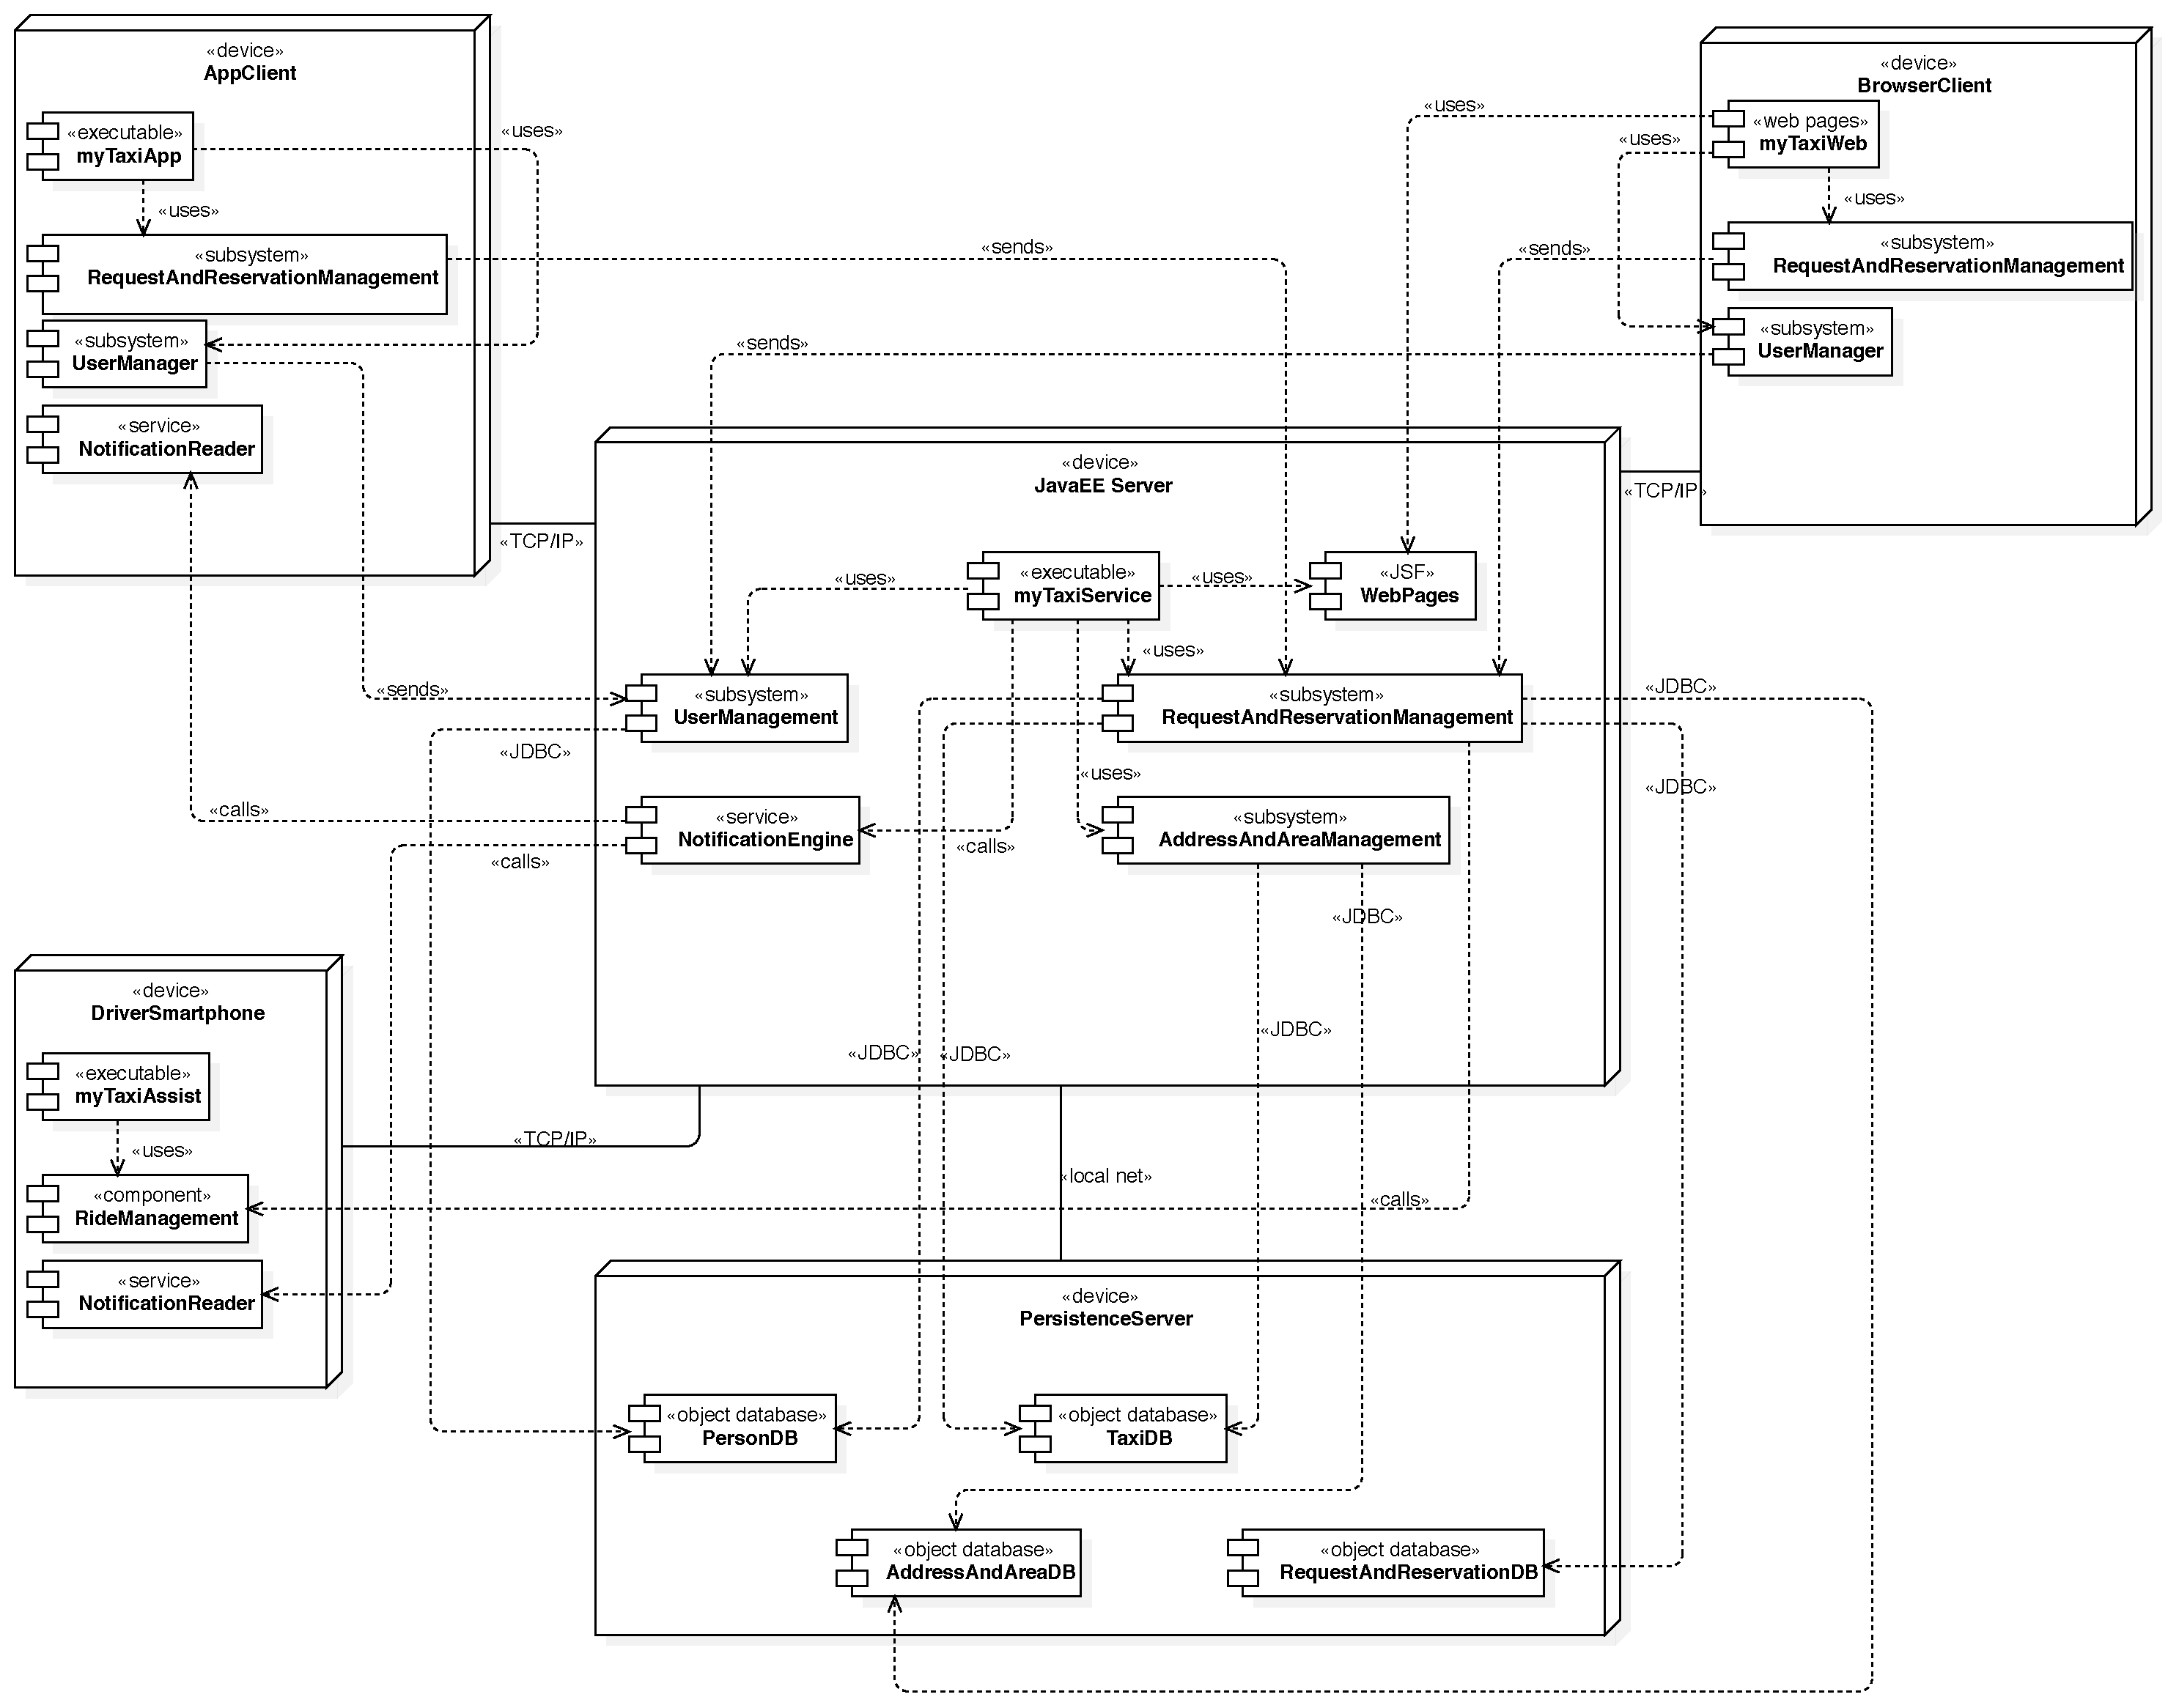
\includegraphics[width=\textwidth]{img/Deploy__DeploymentDiagram_4}
	\caption{Deployment diagram.}
	\label{img:deployment}
\end{figure*}











\clearpage%TODO Remove.
\section{Runtime view}\label{sec:runtime}
[You can use sequence diagrams to describe the way components interact to accomplish specific tasks typically related to your use cases.]
[check SWIM project]
[this is what you have in slide 9 plus sequence diagrams describing the way components behave in order to accomplish a certain activity]

Qui si è voluta presentare una visione delle istanze che possono essere attive sul sistema quando sono state effettuate due richieste, una tramite prenotazione (app) ed una diretta (web) alle quali per comodità è stato allocato lo stesso taxi (ipotizzate consecutive).
Alcune delle relazioni tra le istanze sono date per scontate per motivi di leggibilità (ad esempio il customer della reservation1 (customer1) è lo stesso della request1, ma non viene esplicitato alla request1).


\begin{figure*}
	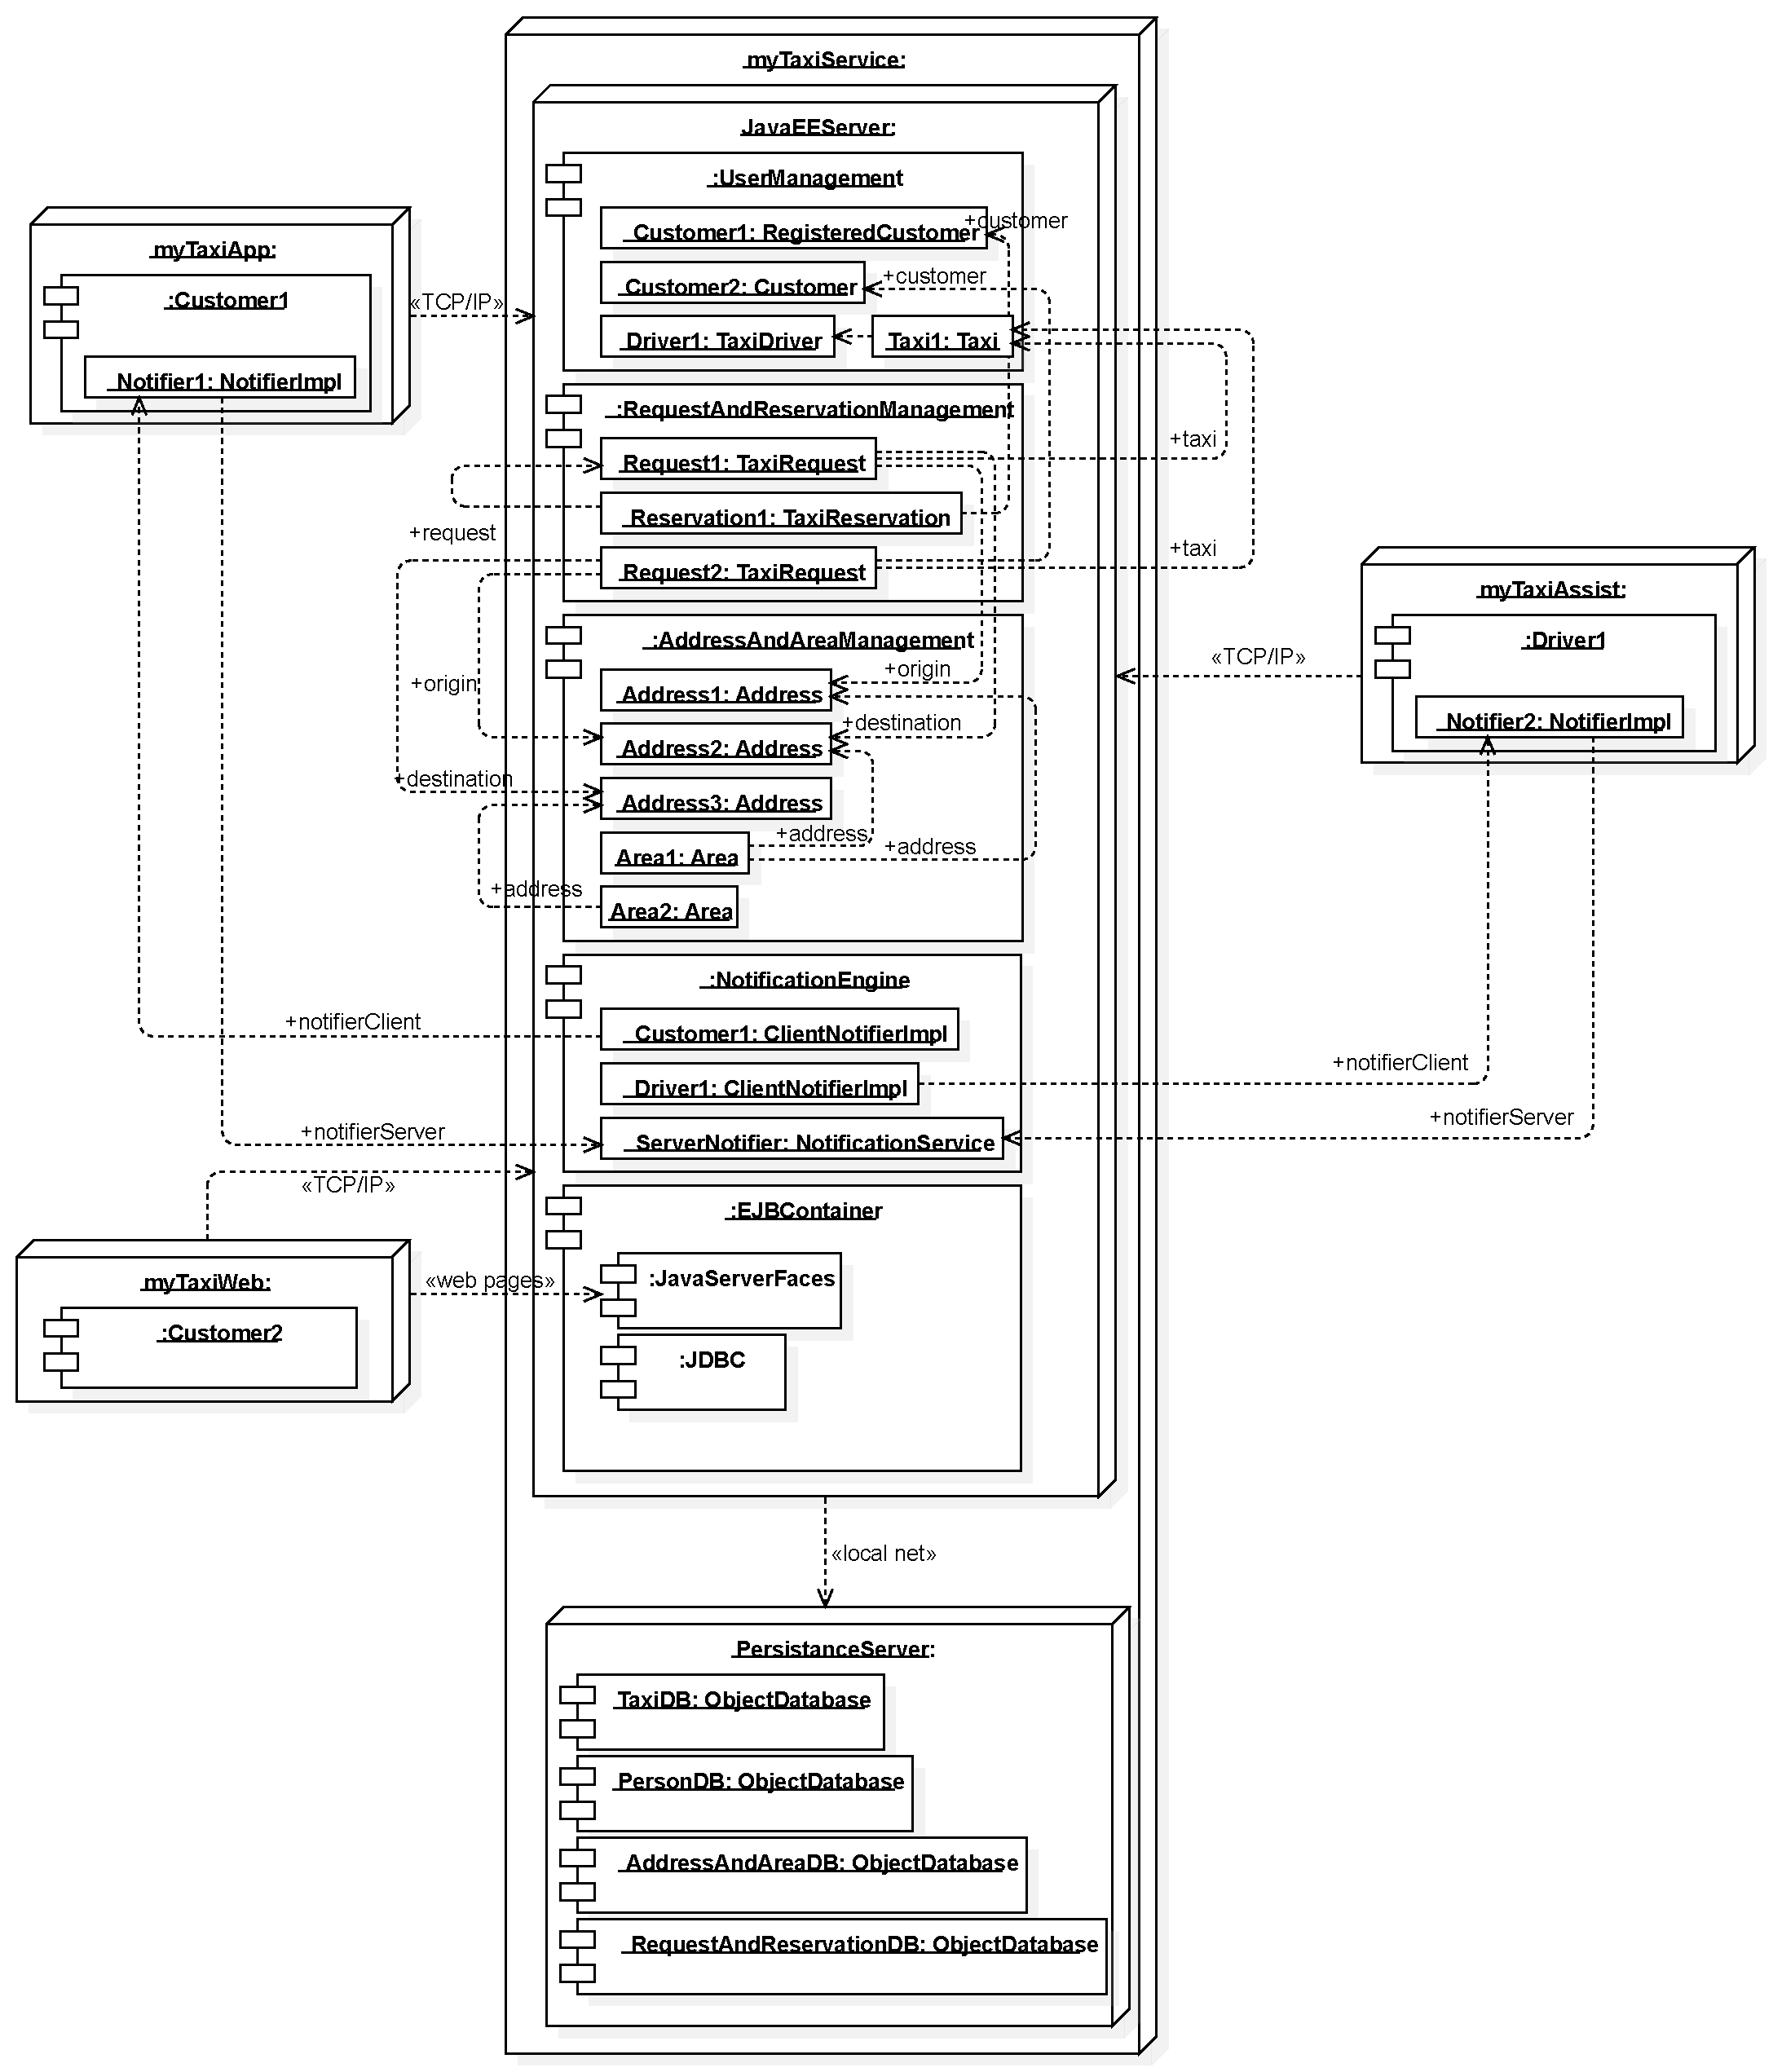
\includegraphics[width=\textwidth]{img/Runtime__RuntimeView_5}
	\caption{Runtime view.}
	\label{img:runtime}
\end{figure*}



SEQUENCE

Questi diagrammi vogliono evidenziare il comportamento del sistema in due casi tipici (una richiesta ed una prenotazione), evidenziando gli scambi di messaggi e i metodi invocati tra i vari component del sistema.



\begin{figure*}
	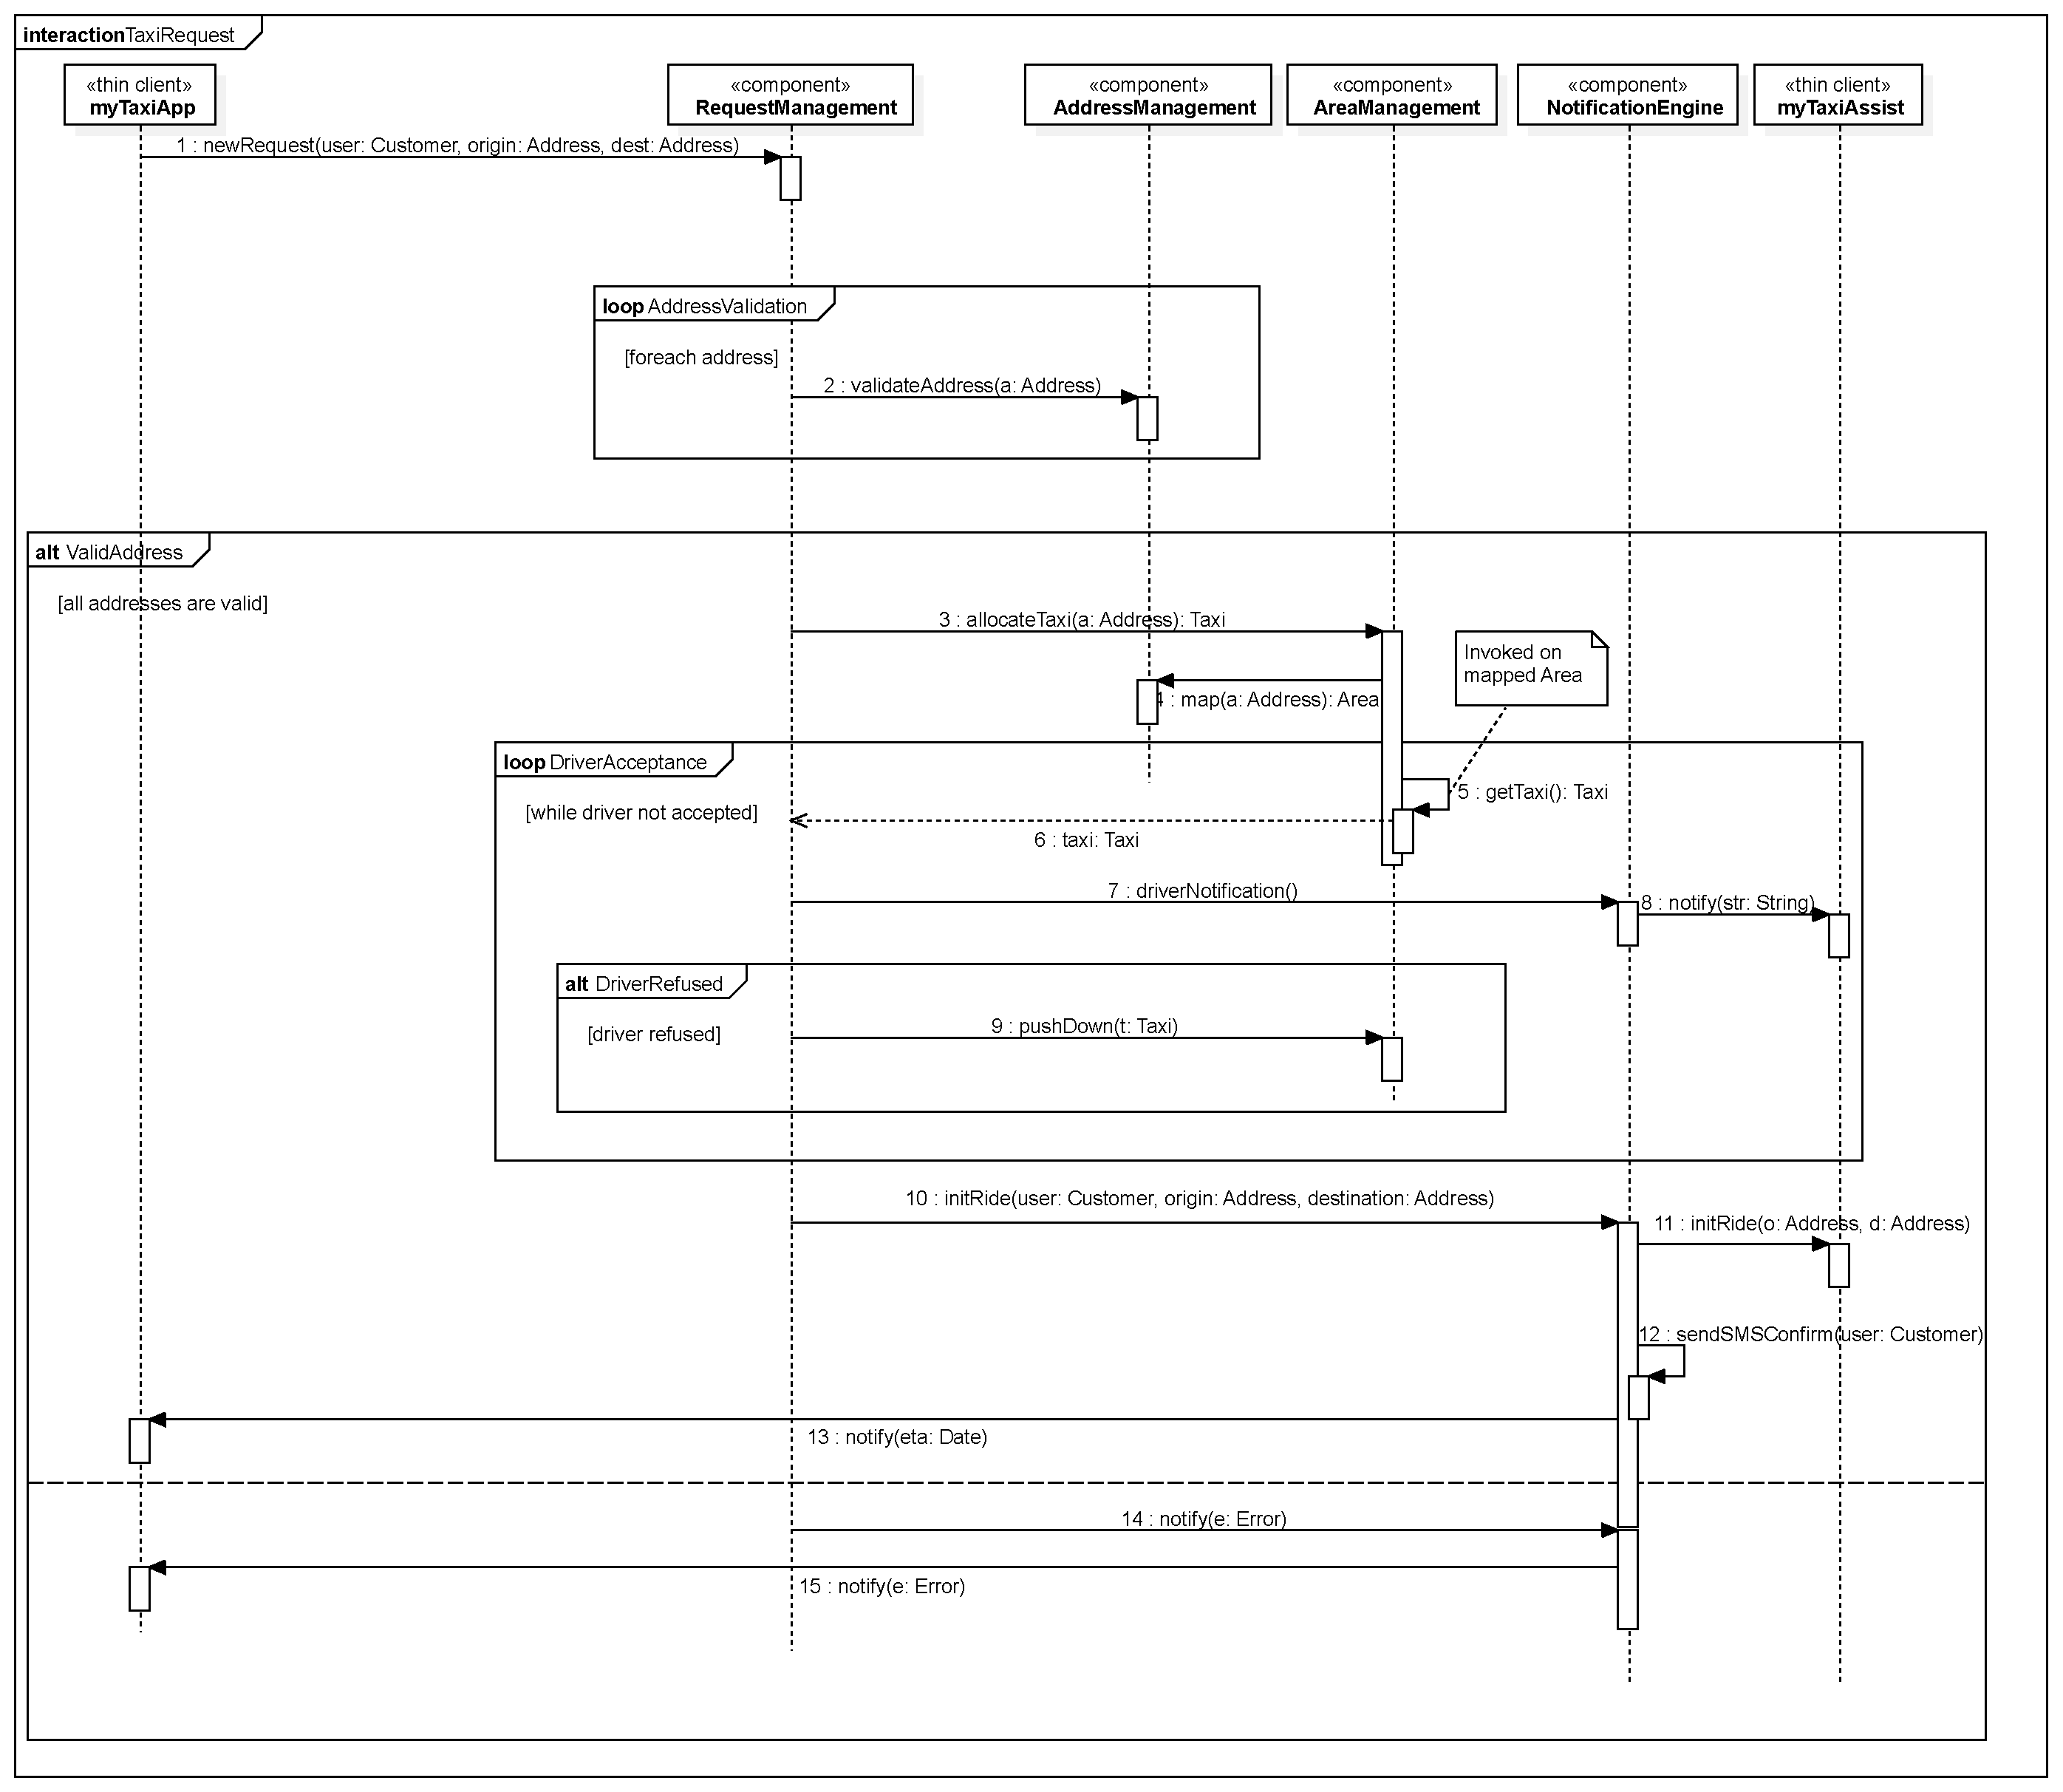
\includegraphics[width=\textwidth]{img/Sequence__Collaboration1__Interaction1__TaxiRequest_2}
	\caption{Taxi request sequence diagram.}
	\label{img:reqSequence}
\end{figure*}

\begin{figure*}
	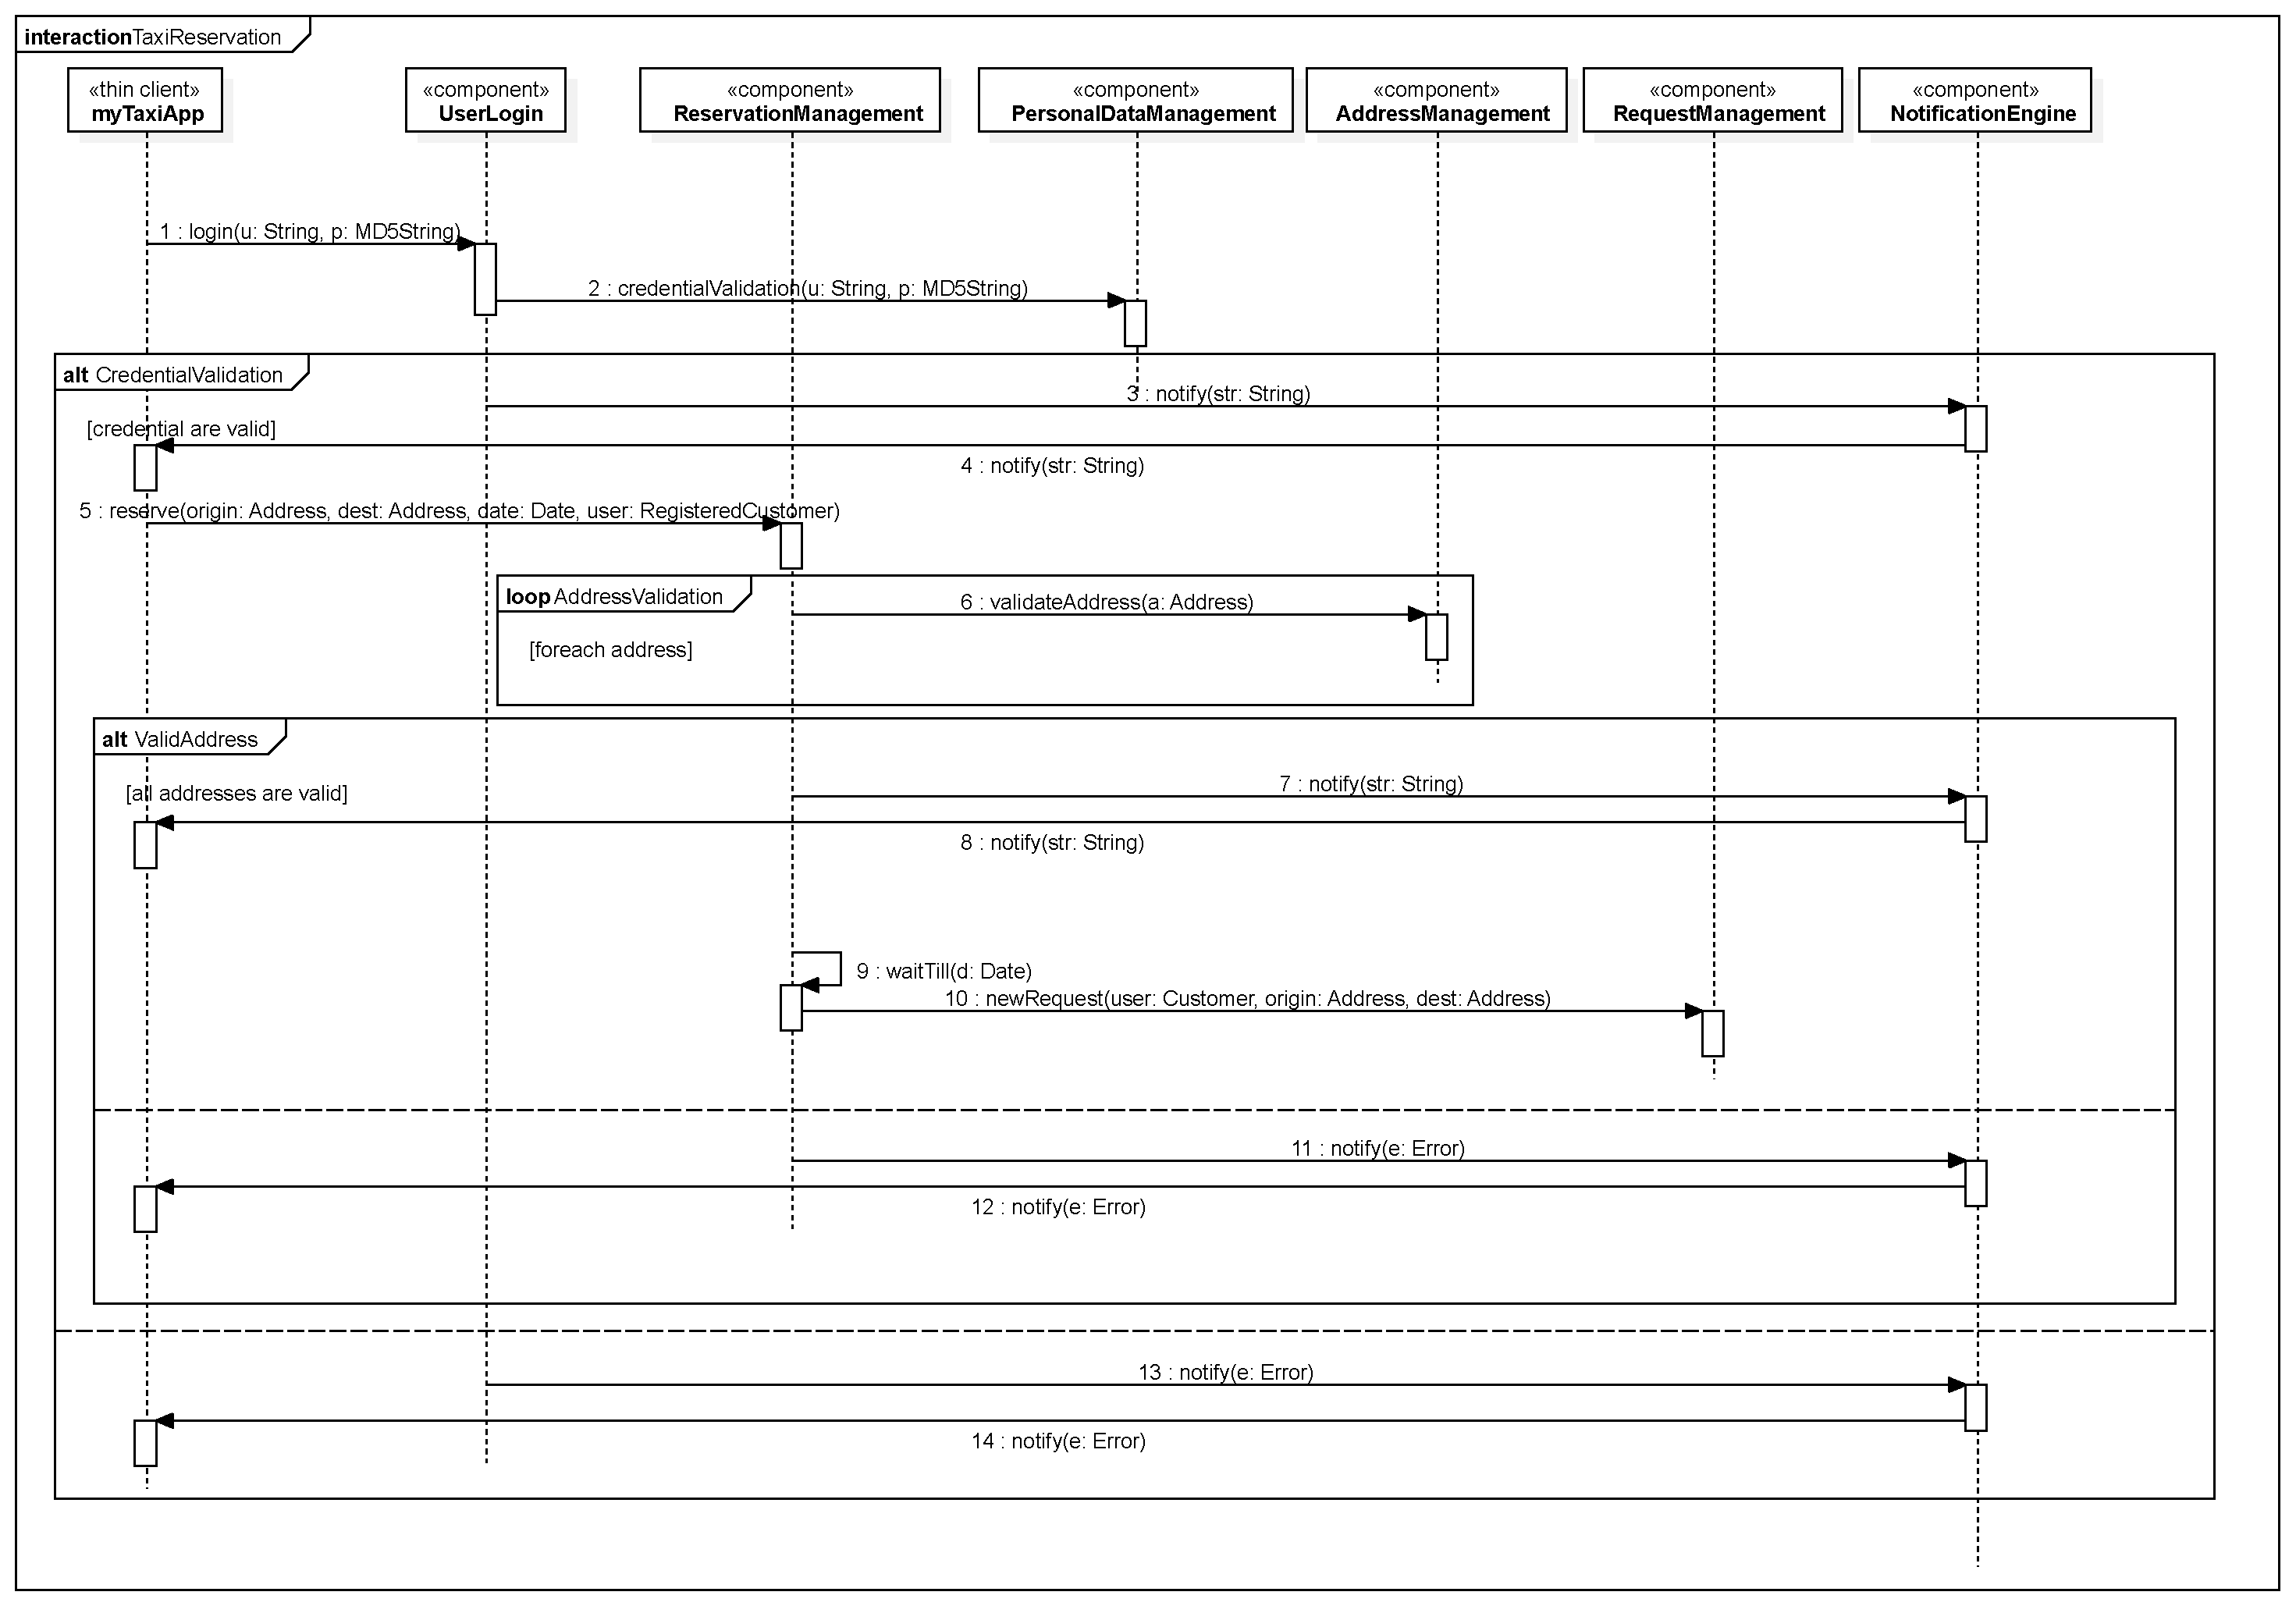
\includegraphics[width=\textwidth]{img/Sequence__Collaboration2__Interaction1__TaxiReservation_3}
	\caption{Taxi reservation sequence diagram.}
	\label{img:resSequence}
\end{figure*}










\clearpage%TODO Remove.
\section{Component interfaces}\label{sec:componentInterfaces}
[communication between components]
[here you define the interfaces of your components, that is, which operations they offer to the external world, their meaning, any input and output parameter (name, possible set of values/type)]














\clearpage%TODO Remove.
\section{Selected architectural styles and patterns}\label{sec:styles}
[Please explain which styles/patterns you used, why, and how.]
[3-tier architecture STYLE; ]















\clearpage%TODO Remove.
\section{Other design decisions}\label{sec:decisions}
\lipsum[8]
